\vspace{-2pt}
\section{Preliminaries}
\label{sec:pre}

To set the stage of our proposed MAAR platform evaluation and DSE, this section introduces the target platform and the evaluation method for a single application on a platform.


%\vspace{-4pt}
\subsection{Target Platform}

ACC-rich platforms include hardware accelerators (ACCs) and programmable processors (CPU, GPU, DSP). \figref{fig:plat} illustrates the target platform for the context of this work. A streaming application $A, B, C, D$ is mapped across SW and HW. Each ACC has a dedicated \newtext{Scratch Pad Memory (SPM)}. All ACCs are aggregated to a HW partition with a shared SPM across all ACCs. ACCs can communicate with each other, and their communication traffic is hidden from system communication fabric (e.g., $B$, $C$). For simplicity, we assume direct n:n communication within the HW partition. Conversely, ACCs and SW kernels communicate through the system streaming fabric (e.g., $A$ to $B$, and $C$ to $D$) which results in throughput penalties.

\vspace{-2pt}
\begin{figure}[h]
	\centering
	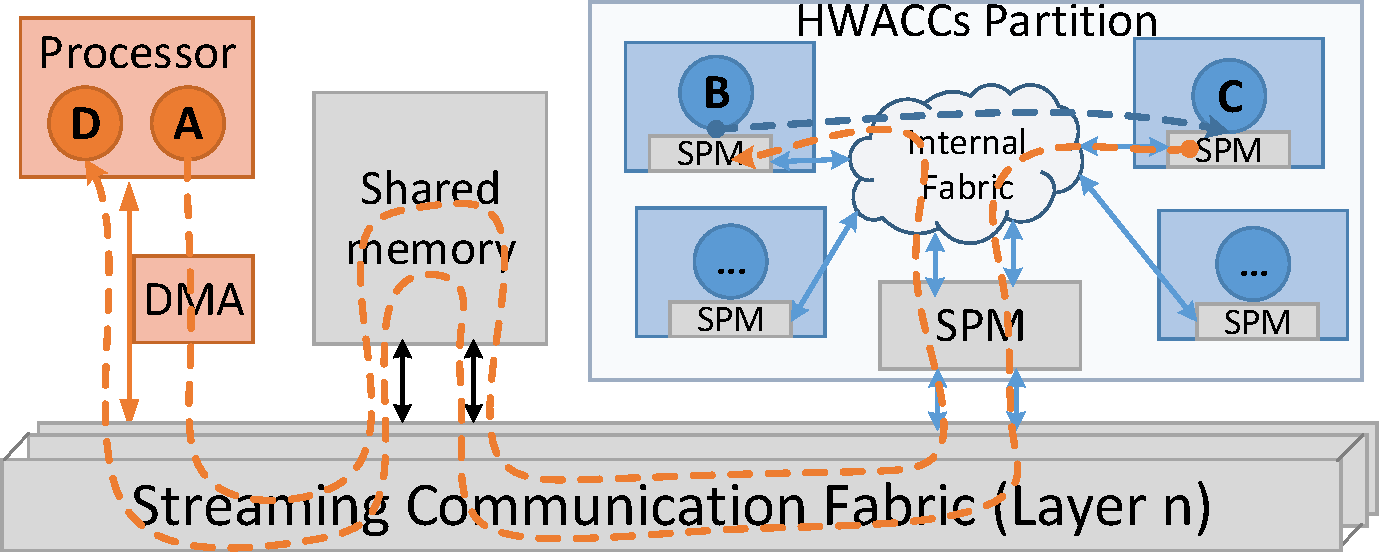
\includegraphics[width=.8\linewidth]{fig/pPlat.pdf}
	\vspace{-4pt}
	\caption{Target Platform}
	\label{fig:plat}
\end{figure}


\vspace{-2pt}
\subsection{Analytic Evaluation}
\label{subsec:ana}

Evaluating an individual application on a platform follows a speed/accuracy trade-off.
The evaluation request in many-application platform design is vast due to (a) the enormous domain design space which needs to be traversed (b) the number of applications which must be evaluated for each allocation. 
An abstract and dramatically fast evaluation, analytic evaluation, is desired to evaluate many more points at the cost of accuracy.

%\begin{figure}[h]
%	\centering
%	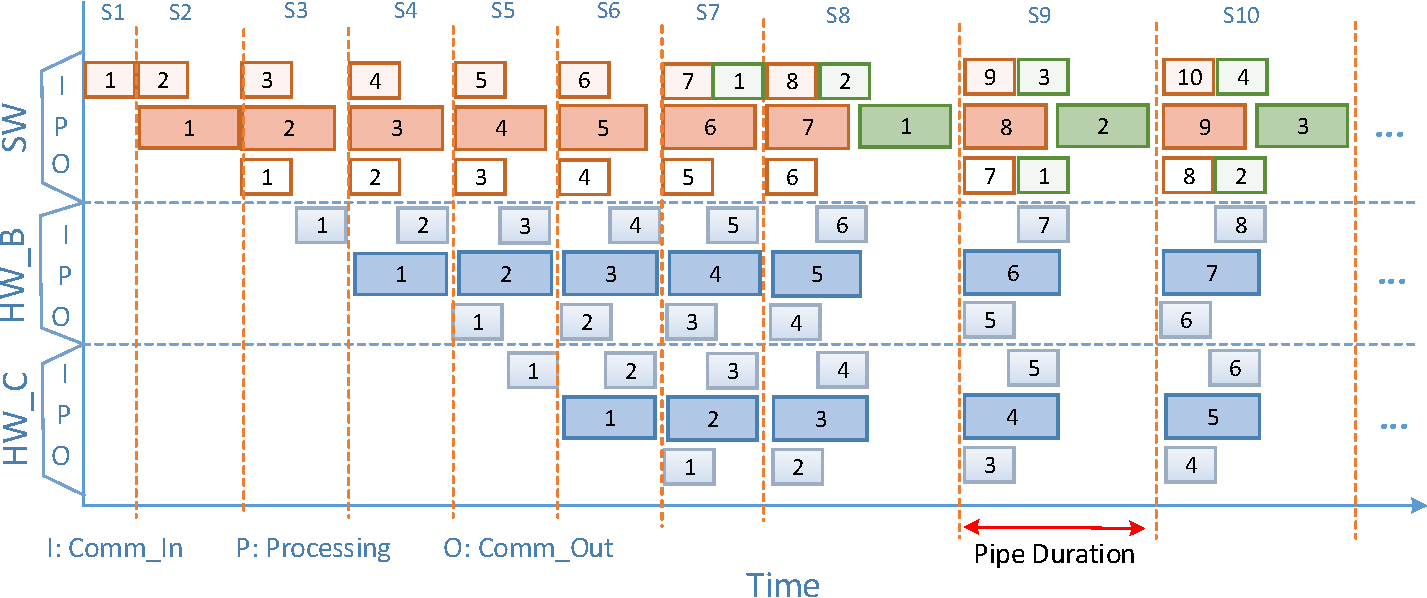
\includegraphics[width=\linewidth]{fig/pPipe.pdf}
%	\caption{Timing diagram of Architecture}
%	\label{fig:Pipe}
%\end{figure}

In analytic evaluation~\cite{Teimouri_TCAD_2018}, the kernels in a streaming application operate as producers and consumers of the streaming data and form a pipeline. 
%\figref{fig:Pipe} visualizes the pipeline execution for two ACCs and one SW core. 
Each pipe stage overlaps communication (in/out) with processing due to double buffering. Actors execute concurrently given their dependencies across different processing components. Actors mapped to the same component execute sequentially.
Our Analytic Evaluation model computes the throughput ($Th$), latency ($L$) and energy consumption ($EC$) of an application based on the inter-kernel pipelined execution.
\newtext{Compared with virtual platforms evaluation generated by the System-on-Chip Environment (SCE) \cite{SCE}, the performance fidelity of Analytic Evaluation is 98\%.}

